\chapter{Hemodynamics}
Hemodynamics explains the movement or flow of the blood. It is influenced by parameters like blood pressure, blood volume, cardiac output, blood composition and viscosity, elasticity of the vessels and lumen of the vessels. It is possible to measure some of the hemodynamic parameters non-invasive, and also to calculate parameters.

\section{Physiological Base}
The regulation of the blood pressure happens with baroreceptors in the wands og the big arteries in chest and neck area. These receptors register the changes of the elongation of the vessels and transmit this information to medulla oblongata. With the received pressure informations  initiates the medulla oblongata, if necessary, regulatory measures. For the short-term regulation is the sympathicus responsible. Both, middle-term and long-term regulation, is made by the kidneys. For middle-term regulation messenger substance are released, which entail vasoconstriction. The long-term regulation occurs  per pressure diuresis or reabsorption in the kidneys.\\

It is possible to measure different blood pressures at different places in the cardiovascular system, for example the mean arterial pressure. The $ MAP $ increases with ejection of the stroke volume and decreases with outflow if the blood in the periphery. The central venous pressure states the pressure in the venous system and complies approximately the pressure in the right ventricle. $ CVP $ depends on the filling volume of the venous system.

Effects on the blood pressure have cardiac output, total periphery resistance and the viscosity of the blood.\\

The cardiac output $ CO $ states the blood volume, which is pumped by the heart per time unit. The calculation of the $ CO $ as follows.\\

$ CO=HF\times stroke volume $\\

The total periphery resistance is the flow resistance of the systemic circulation and results from the sum of all vessel resistances. $ TPR $ depends on $ MAP $ , $ CVP $ and $ CO $.\\

$ TPR=\frac{MAP-CVP}{CO} $

\section{Physical Base}
To consider the hemodynamics, it is possible to draw conclusions by analogy of physical laws. Especially of Ohm's law $ R=\frac{U}{I} $ or rather $ I=\frac{U}{R} $.\\

A special case of Ohm's law constitutes Hagen-Poiseuille's law in the field of fluid dynamic and rheology. Hagen-Poiseuille's law describes the laminar flow of an homogeneous Newtonian fluid through a rigid pipe depending on characteristics of the fluid and of the pipe.

Blood is an inhomogeneous suspension of liquid and corpuscular components, whose viscosity $ \eta $ depends on more factors than the temperature, and is consequently no Newtonian fluid. Nevertheless it is possible to draw conclusions by analogy out of Hagen-Poiseuille's law for the computation of the hemodynamics.\\

$ \frac{V}{t}=\frac{r^{4}\times\pi\times\Delta P}{8\times\eta\times I} $\\

Here is the volume flow equivalent to the electrical current $ I $ and the pressure difference $ \Delta $P to the electric Voltage $ U $. Thus, the calculation of the Resistance as follows.\\

$ R=\frac{8\times I\times\eta}{r^{4}} $\\

The logical conclusion is, that the volume flow increases 16 times and the resistance decreases 16 times for double radius $ r $.\\

In the blood is the oxygen tied to a large extent by hemoglobin. The oxygen saturation describes the percentage of the oxygenated hemoglobin. With rising oxygen partial pressure increases the oxygen saturation. This relation between $ sO_{2} $ and $ pO_{2} $ is showed by the oxygen binding curve.

\begin{figure}[H]                                         %   File-type can be specified
	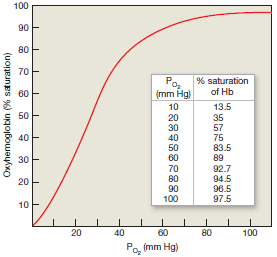
\includegraphics[width=.4\textwidth]{figures/oxygen_saturation_curve}  %<--but is not needed.
	\caption{This image is clearly too small, remember to scale appropriately \fxnote{Remember source}}
	\label{fig:FigureLABEL}  %<--give the figure a label, so you can reference!
\end{figure}

The oxygen content of the blood depends on both, the oxygen saturation and the oxygen partial pressure. $ cO_{2} $ is calculated by the sum of the hemoglobin bounded and the physical dissolved oxygen.\\

$ cO_{2}=Hb\times 1,34\frac{ml}{g} + pO_{2}\times 0,003\frac{ml\times dl}{mmHg} $\\

The available oxygen is calculates by the oxygen content of the blood and the cardiac output.\\

$ DO_{2}=cO_{2}\times CO $\\

The consumption of oxygen is calculated by the difference between the available oxygen in the arterial and the venous blood and the cardiac output.\\

$ VO_{2}=(c_{a}O_{2}-c_{v}O_{2})\times CO $\\

Therefore one can draw a conclusion from the available and the consumption of oxygen to the cardiac output.